\textbf{\Large Grundlagen}\\

Das ventilatorische Schwellenkonzept basiert auf der physiologischen Reaktion des Körpers auf die zunehmende Belastung bei einer Spiroergometrie. Da der Muskelgehalt des körpereigenen Energiestoffs ATP zur Muskelkontraktion nur für eine kurze Zeit ausreicht, muss dieser für andauernde Arbeit durch Glykolyse resynthetisiert werden \cite{Kroidl.2015}. Reicht ab einer bestimmten Belastung die Sauerstoffaufnahme (\.{V}O\textsubscript{2}) nicht mehr aus, funktionieren gewisse, für die Glykolyse notwendige Coenzyme nicht mehr, sodass in den Muskeln Laktat akkumuliert und es allmählich zur metabolischen Azidose (Übersäuerung) kommt. Der Körper kompensiert dies durch Puffer-Reaktionen, wodurch überschüssiges Kohlenstoffdioxid (CO\textsubscript{2}) anfällt, welches abgeatmet wird und respiratorisch gemessen werden kann.\\
Nach einer Spiroergometrie werden Atemparameter grafisch verglichen, um ventilatorische Reaktionen auf biochemische Prozesse zu detektieren. Die ventilatorischen Schwellen stellen Stoffwechselübergänge dar, anhand derer mit verschiedenen Modellen Trainingsbereiche bestimmbar sind. Sie werden für üblich als Herzfrequenz in \si{\per\minute} angegeben. Die VT1 wird mittels der V-Slope-Methode oder anhand des Sauerstoff-Äquivalents (EQO\textsubscript{2}) grafisch identifiziert. Das Kohlenstoffdioxid-Äquivalent (EQCO\textsubscript{2}) oder der Vergleich der Ventilation (\.{V}E) zur Kohlenstoffdioxidabgabe (\.{V}CO\textsubscript{2}) eignen sich zur Bestimmung der VT2.\\

\begin{picture}(\spaltenbreite,6)
\put(0.9,2){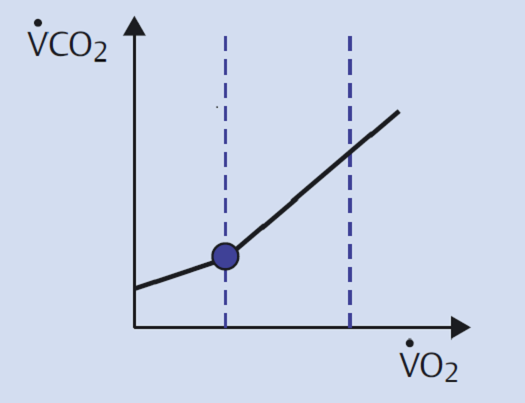
\includegraphics[width=50mm]{Bilder/vslope.png}}
\put(1.6,0.7){\parbox{720pt}{{\bf \small a):} \small V-Slope}}
\put(7.1,2){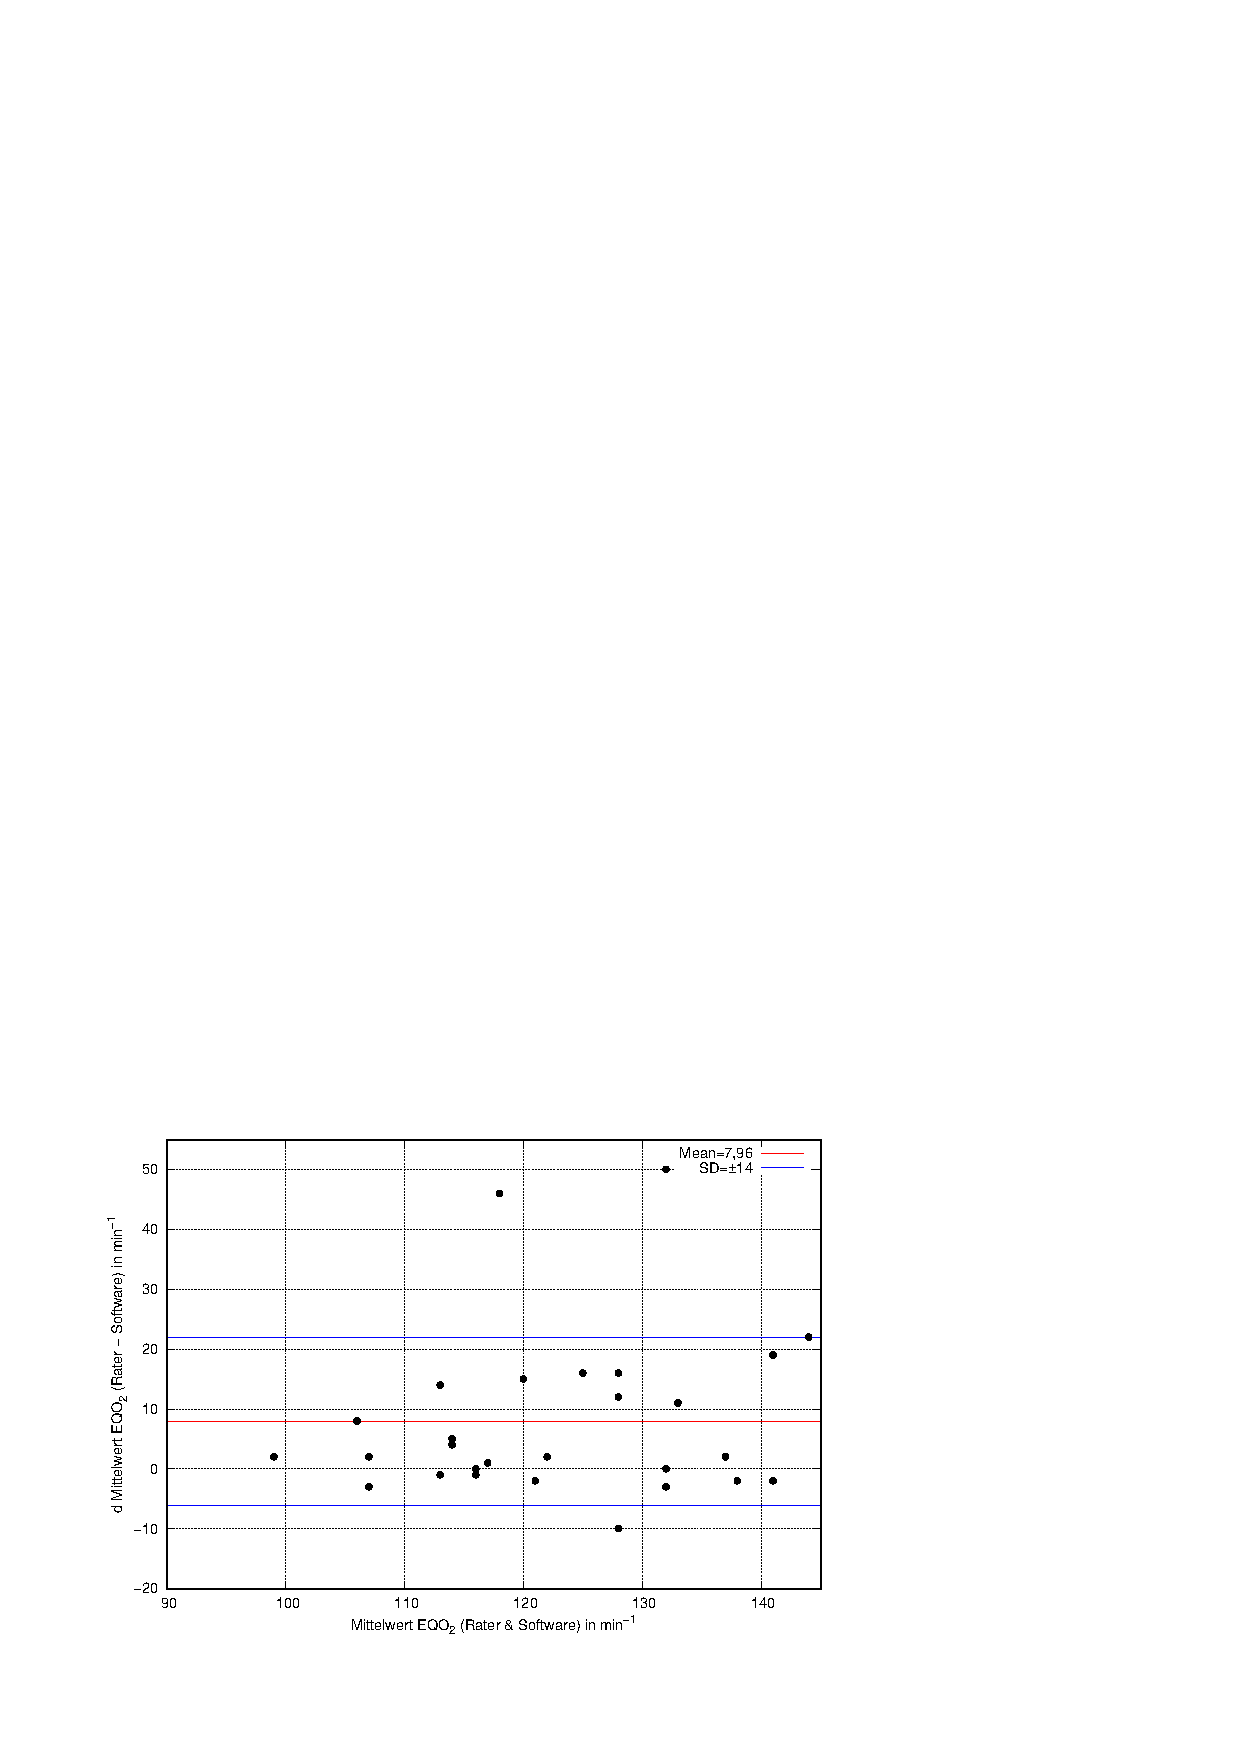
\includegraphics[width=50mm]{Bilder/eqo2.png}}
\put(8.1,0.7){\parbox{720pt}{{\bf \small b)} \small EQO\textsubscript{2}}}
\put(13.3,2){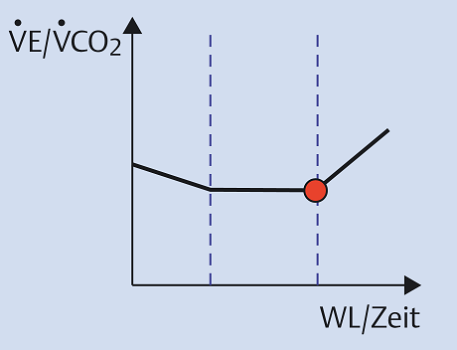
\includegraphics[width=50mm]{Bilder/eqco2.png}}
\put(14.1,0.7){\parbox{720pt}{{\bf \small c)} \small EQCO\textsubscript{2}}}
\put(19.6,2){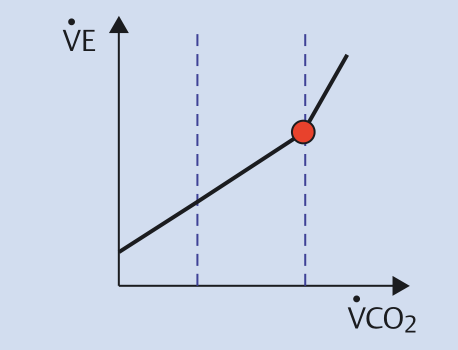
\includegraphics[width=50mm]{Bilder/field4.png}}
\put(20.1,0.78){\parbox{720pt}{{\bf \small d)} \small \.{V}E/\.{V}CO\textsubscript{2}}}
\put(1.4,-0.6){\parbox{720pt}{{\bf \small Abb. 1:} \small Methoden zur Schwellenbestimmung: VT1: blau; VT2: orange}}
\end{picture}
